\setlength{\parskip}{0.125in}

\chapter{Объявление о проведении Конкурса}

Общество с ограниченной ответственностью <<Мэйл.Ру>>, созданное и действующее в соответствии с законодательством Российской Федерации, с
местом нахождения по адресу: 125167, г. Москва, Ленинградский проспект, д. 39, строение 79, далее по тексту <<Организатор конкурса>>,
приглашает физических лиц, достигших к моменту опубликования настоящего Объявления о конкурсе 18 лет, далее по тексту <<Участник конкурса>>,
к участию в конкурсе на нижеследующих условиях:

\section{Наименование Конкурса}

<<Российский кубок по программированию искусственного интеллекта (Russian AI Cup)>>.

Целями проведения Конкурса являются:
\begin{itemize}
\item повышение общественного интереса к сфере создания программных продуктов;
\item предоставление Участникам конкурса возможности раскрыть творческие способности;
\item развитие профессиональных навыков Участников конкурса.
\end{itemize}

Конкурс состоит из 3 (трёх) этапов, каждый из которых завершается определением Победителей. Последний этап Конкурса является решающим для
Участников конкурса в состязании за получение звания Победителя Конкурса, занявшего соответствующее призовое место.

\section{Информация об организаторе конкурса}

Наименование: ООО <<Мэйл.Ру>>

Адрес места нахождения: 125167, г. Москва, Ленинградский проспект, д. 39, строение 79

Почтовый адрес: 125167, г. Москва, Ленинградский проспект, д. 39, строение 79, БЦ <<SkyLight>>

Телефон: (495) 725-63-57

Сайт: http://www.russianaicup.ru

Е-мейл: russianaicup@corp.mail.ru

\section{Сроки проведения Конкурса}

Срок проведения Конкурса: с 00.00 часов 8 сентября 2014 года до 24.00 часов 19 октября 2014 года по Московскому времени.

Сроки начала и окончания этапов Конкурса:
\begin{itemize}
\item первый этап – с 00 часов 00 минут 27 сентября 2014 года до 24 часов 00 минут 28 сентября 2014 года;
\item второй этап – с 00 часов 00 минут 4 октября 2014 года до 24 часов 00 минут 5 октября 2014 года;
\item третий этап (заключительный) – с 00 часов 00 минут 11 октября 2014 года до 24 часов 00 минут 12 октября 2014 года.
\end{itemize}

\section{Условие получения статуса Участника конкурса}

Для участия в Конкурсе необходимо пройти процедуру регистрации в Системе Организатора конкурса, размещённой на сайте Организатора конкурса в
сети Интернет по адресу: http://www.russianaicup.ru.

\section{Срок регистрации Участников конкурса в Системе Организатора}

Регистрация Участников конкурса проводится с 00.00 часов 8 сентября 2014 года до 24.00 часов 19 октября 2014 года включительно.

\section{Территория проведения Конкурса}

Конкурс проводится на территории Российской Федерации. Проведение всех этапов Конкурса осуществляется путем удалённого доступа к Системе
Организатора конкурса через сеть Интернет.

\section{Условия проведения Конкурса (существо заданий, критерии и порядок оценки)}

Порядок проведения Конкурса, существо задания, критерии и порядок оценки указаны в конкурсной документации в разделе 2.1.

Конкурсная документация включает в себя:
\begin{itemize}
\item Объявление о проведении Конкурса;
\item Соглашение об организации и порядке проведения Конкурса;
\item Правила проведения Конкурса;
\item информационные данные, содержащиеся в Системе Организатора конкурса.
\end{itemize}

Участник конкурса может ознакомиться с конкурсной документацией на сайте Организатора конкурса в сети Интернет по адресу:
http://www.russianaicup.ru, а также при прохождении процедуры регистрации в Системе Организатора конкурса.

Организатор конкурса оставляет за собой право на изменение конкурсной документации, условий проведения Конкурса и отказ от его проведения в
соответствии с условиями конкурсной документации и нормами законодательства РФ. При этом, Организатор Конкурса обязуется уведомить
Участников конкурса обо всех произошедших изменениях путём отправки уведомления, в порядке и на условиях, предусмотренных в конкурсной
документации.

\section{Порядок определения Победителей и вручения Призов. Призовой фонд Конкурса}

Критерии оценки результатов Конкурса, количество и порядок определения Победителей содержатся в разделе 2.1 данного документа.

Призовой фонд Конкурса формируется за счет средств Организатора конкурса.

Призовой фонд:
\begin{itemize}
\item 1 место --- Apple Mac Pro;
\item 2 место --- Apple Macbook Pro 13.3\textquotedbl;
\item 3 места --- Apple Macbook Air 13.3\textquotedbl;
\item 4-8 места --- Apple iPad mini 7.9\textquotedbl 16GB Wi-Fi;
\item 1-6 места в квалификации (Песочница) --- Apple iPod nano 16GB.
\end{itemize}

Все участники Конкурса, принявшие участие во втором или третьем этапах, будут вознаграждены футболкой.

Все участники, занявшие призовые места, будут оповещены посредством отправки сообщения на адрес электронной почты, указанный участником при
регистрации в Системе Организатора. 

Призы будут высланы участникам в виде посылок, используя Почту России, в течение двух месяцев после окончания финального этапа. Срок
доставки приза по почтовому адресу, указанному участником, зависит от сроков доставки Почты России. Почтовые адреса призёров для отправки
призов Организатор получает из учётных данных участника в Системе Организатора. Адрес должен быть указан участником-призёром в течение трёх
дней после получения уведомления о получении приза.

При отсутствии ответа в обозначенные сроки или отказе предоставить точные данные, необходимые для вручения призов Конкурса, Организатор
оставляет за собой право отказать такому участнику в выдаче приза Конкурса. Денежный эквивалент приза не выдаётся.
 
Победители Конкурса обязуются предоставить Организатору конкурса копии всех документов, необходимых для бухгалтерской и налоговой отчетности
Организатора конкурса. Перечень документов, которые Победитель обязан предоставить Организатору конкурса, включает в себя:
\begin{itemize}
\item копию паспорта Победителя;
\item копию свидетельства о постановки на налоговый учет Победителя;
\item копию пенсионного удостоверения Победителя;
\item данные об открытии банковского лицевого счета Победителя;
\item иные документы, которые Организатор конкурса потребует от Участника конкурса в целях формирования отчётности о проведённом Конкурсе.
\end{itemize}

Наряду с копиями Организатор конкурса вправе запросить оригиналы вышеуказанных документов.

В соответствии с подпунктом 4 пункта 1 статьи 228 НК РФ Победитель Конкурса, ставший обладателем Приза, самостоятельно несёт все расходы по
уплате всех применимых налогов, установленных действующим законодательством Российской Федерации.

\section{Порядок и способ информирования участников Конкурса}

Информирование Участников Конкурса осуществляется путём размещения информации в сети Интернет на Сайте Организатора конкурса по адресу:
http://www.russianaicup.ru, а также через Систему Организатора конкурса, в течение всего срока проведения Конкурса.

\chapter{О мире CodeHockey 2014}

\section{Общие положения игры и правила проведения турнира}

Данное соревнование предоставляет вам возможность проверить свои навыки программирования, создав искусственный интеллект (стратегию),
управляющий командой хоккеистов в специальном игровом мире (подробнее об особенностях мира CodeHockey 2014 можно узнать в следующих
разделах). В зависимости от этапа соревнования у вас в команде будет от $2$ до $6$ полевых хоккеистов (при этом одновременно на площадке
может находиться не более трёх, остальные должны сидеть на скамейке запасных), а также вратарь. Полевые хоккеисты могут отличаться друг от
друга по ряду параметров, однако гарантируется, что начальное расположение и параметры хоккеистов симметричны\footnote[1]{Относительно
вертикальной линии, проходящей через центр поля.} для обеих стратегий. Помимо хоккеистов в игре присутствует ещё один тип объектов (юнитов):
это хоккейная шайба. Вратарь перемещается автоматически, пытаясь оставаться на одной горизонтальной линии с шайбой, управлять им вы не
можете.

В каждой игре вам будет противостоять стратегия другого игрока. Как и в настоящем хоккее, ваша команда должна забрасывать шайбу в ворота
противника и мешать попаданию шайбы в свои ворота. Команда, забросившая больше шайб, объявляется победителем. Игра может закончиться и
ничьей, если обе команды забили одинаковое количество голов. Тогда командам назначается дополнительное время. Если к этому моменту не было
забито ни одного гола, то вратари обеих команд убираются из игрового мира. Первый же гол, забитый в дополнительное время, определяет
победителя, игра при этом завершается. Команды могут подтвердить ничью, если за дополнительное время не будет заброшено ни одной шайбы.

Турнир проводится в несколько этапов, которым предшествует квалификация в Песочнице. Песочница --- соревнование, которое проходит на
протяжении всего чемпионата. В рамках каждого этапа игроку соответствует некоторое значение рейтинга --- показателя того, насколько успешно
его стратегия участвует в играх.

Начальное значение рейтинга в Песочнице равно $1200$. По итогам игры это значение может как увеличиться, так и уменьшиться. При этом победа
над слабым (с низким рейтингом) противником даёт небольшой прирост, также и поражение от сильного соперника незначительно уменьшает ваш
рейтинг. Если победа или поражение произошли в дополнительное время, то рейтинг меняется значительно меньше обычного. Со временем рейтинг в
Песочнице становится всё более инертным, что позволяет уменьшить влияние случайных длинных серий побед или поражений на место участника,
однако вместе с тем и затрудняет изменение его положения при существенном улучшении стратегии. Для отмены данного эффекта участник может
сбросить изменчивость рейтинга до начального состояния при отправке новой стратегии, включив соответствующую опцию. В случае принятия новой
стратегии системой рейтинг участника мгновенно упадёт, однако по мере участия в играх быстро восстановится и даже станет выше, если ваша
стратегия действительно стала эффективнее.

Начальное значение рейтинга на каждом основном этапе турнира равно $0$. За каждую игру участник получает определённое количество единиц
рейтинга в зависимости от занятого в ней места. А именно:
\begin{itemize}
\item За победу в основное время участник получает $3$ единицы рейтинга, его противник получает $0$.
\item За победу в дополнительное время участник получает $2$ единицы рейтинга, его противник получает $1$.
\item За ничью оба участника получают по $1$ единице рейтинга.
\end{itemize}

Сначала все участники могут участвовать только в играх, проходящих в Песочнице. Игроки могут отправлять в Песочницу свои стратегии, и
последняя принятая из них берётся системой для участия в квалификационных играх. Каждый игрок участвует примерно в $1$ квалификационной игре
за час. Жюри оставляет за собой право изменить этот интервал, исходя из пропускной способности тестирующей системы, однако для всех игроков
он остаётся постоянной величиной. Игры в Песочнице проходят по правилам, соответствующим правилам случайного прошедшего этапа турнира или же
правилам следующего (текущего) этапа. При этом, чем ближе значение рейтинга двух игроков в рамках Песочницы, тем больше вероятность того,
что они окажутся в одной игре. Песочница стартует до начала первого этапа турнира и завершается через некоторое время после финального
(смотрите расписание этапов для уточнения подробностей). Помимо этого Песочница замораживается на время проведения этапов турнира. По итогам
игр в Песочнице происходит отбор для участия в Раунде $1$, в который пройдут $900$ участников с наибольшим рейтингом (при его равенстве
приоритет отдаётся игроку, раньше отправившему последнюю версию своей стратегии).

Этапы турнира:
\begin{itemize}
  \item Раунд $1$ проверит ваши навыки управления командой из двух хоккеистов. Этап пройдёт по упрощённым правилам, о чем подробнее читайте
        далее. Этот этап, как и все последующие, состоит из двух частей, между которыми будет небольшой перерыв (с возобновлением работы
        Песочницы), который позволит улучшить свою стратегию. Для игр в каждой части выбирается последняя стратегия, отправленная игроком
        до начала части. Игры проводятся волнами. В каждой волне каждый игрок участвует ровно в одной игре. Количество волн в каждой части
        определяется возможностями тестирующей системы, но гарантируется, что оно не будет меньше десяти. $300$ участников с наиболее
        высоким рейтингом пройдут в Раунд $2$. Также в Раунд $2$ будет проведён добор $60$ участников с наибольшим рейтингом в Песочнице (на
        момент начала Раунда $2$) из числа тех, кто не прошёл по итогам Раунда $1$.
  \item В играх Раунда $2$ будет участвовать по $3$ хоккеиста с каждой стороны. Участникам придётся не только координировать возросшее
        количество юнитов, но и учитывать разницу между ними: на этом этапе вводится понятие атрибутов хоккеистов. Между этапами будет
        некоторый перерыв, так что у вас есть возможность доработать стратегию. Усложняет задачу то, что после подведения итогов Раунда $1$
        часть слабых стратегий будет отсеяна и вам придётся противостоять более сильным соперникам. По итогам Раунда $2$ лучшие $50$
        стратегий попадут в Финал. Также в Финал будет проведен добор $10$ участников с наибольшим рейтингом в Песочнице (на момент начала
        Финала) из числа тех, кто не прошёл в рамках основного турнира.
  \item Финал является самым серьёзным этапом. После отбора, проведённого по итогам двух первых этапов, останутся сильнейшие. И в каждой
        игре вам придётся сойтись лицом к лицу с одним из них. У игрока в распоряжении находится команда из $6$ хоккеистов, из которых
        одновременно на игровой площадке находятся только трое, а остальные сидят на скамейке запасных. В игру вводится понятие выносливости.
        Немного выносливости тратится на каждое действие хоккеиста. Выносливость восстанавливается сама по себе для всех хоккеистов, но для
        сидящих в запасе скорость восстановления заметно выше. Система проведения Финала имеет свои особенности. Этап по-прежнему делится
        на две части, однако они уже не будут состоять из волн. В каждой части этапа будут проведены игры между всеми парами участников
        Финала. Если позволит время и возможности тестирующей системы, операция будет повторена.
\end{itemize}

После окончания Финала все финалисты упорядочиваются по невозрастанию рейтинга. При равенстве рейтингов более высокое место занимает тот
финалист, чья участвовавшая в финале стратегия была отослана раньше. Призы за Финал распределяются на основании занятого места после этого
упорядочивания. Лучшие восемь финалистов награждаются призами:
\begin{itemize}
\item 1 место --- Apple Mac Pro;
\item 2 место --- Apple Macbook Pro 13.3\textquotedbl;
\item 3 места --- Apple Macbook Air 13.3\textquotedbl;
\item 4-8 места --- Apple iPad mini 7.9\textquotedbl 16GB Wi-Fi.
\end{itemize}

После окончания Песочницы все её участники, кроме призёров Финала, упорядочиваются по невозрастанию рейтинга. При равенстве рейтингов более
высокое место занимает тот участник, который раньше отослал последнюю версию своей стратегии. Призы за Песочницу распределяются на основании
занятого места после этого упорядочивания. Лучшие шесть участников Песочницы награждаются ценными подарками.

\section{Описание игрового мира}

Игровой мир представляет собой некоторую двумерную прямоугольную область. Размер области --- $1200\times800$. Ось абсцисс в этом мире
направлена слева направо, ось ординат --- сверху вниз, угол $0.0$ совпадает с направлением оси абсцисс, а положительный угол вращения
означает вращение по часовой стрелке. Ниже приведены две схемы игровой площадки с начальным расположением команд из двух и из трёх
хоккеистов:

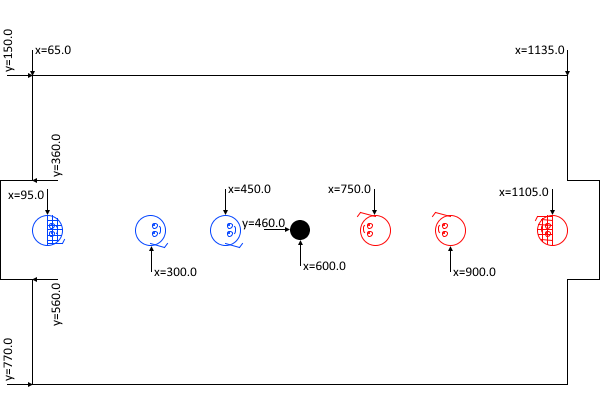
\includegraphics{images/FieldScheme-2vs2-1200x800.png}

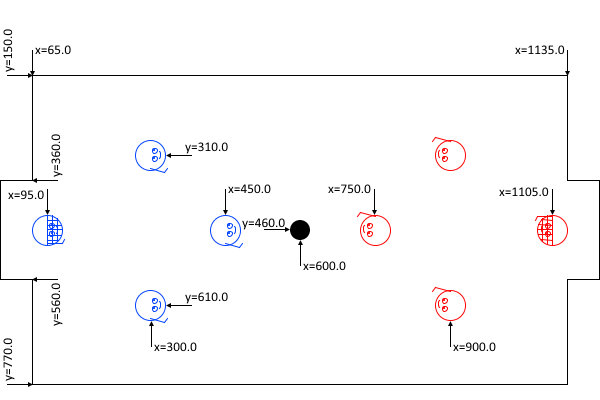
\includegraphics{images/FieldScheme-3vs3-1200x800.png}

Время в игре дискретное и измеряется в <<тиках>>. В начале каждого <<тика>> игра получает от стратегий желаемые действия хоккеистов в этот
тик и обновляет состояние хоккеистов в соответствии с этими желаниями и ограничениями мира. Затем происходит расчёт изменения мира и
объектов в нём за этот тик, и процесс повторяется снова с обновлёнными данными. Базовая длительность каждой игры --- $6000$ тиков.
В случае равного счёта по окончании основного времени игра продлевается на $2000$ тиков дополнительного времени. Помимо этого, игра не может
закончиться в течение $300$ тиков после забитого гола. Эти $300$ тиков являются периодом <<вне игры>>, о чём подробнее читайте в следующем
разделе. Таким образом, максимально возможная длительность игры составляет $8300$ тиков. Если стратегии обоих участников <<упали>>, игра
завершается преждевременно.

<<Упавшая>> стратегия больше не может управлять хоккеистами. Стратегия считается <<упавшей>> в следующих случаях:
\begin{itemize}
  \item Процесс, в котором запущена стратегия, непредвиденно завершился, либо произошла ошибка в протоколе взаимодействия между стратегией
        и игровым сервером.
  \item Стратегия превысила одно (любое) из отведённых ей ограничений по времени. Стратегии на один ход хоккеиста выделяется не более
        $2$ секунд реального времени. Но в сумме на всю игру процессу стратегии выделяется
        \begin{equation}
        50\times\textit{<длительность\_игры\_в\_тиках>}\times\textit{<количество\_хоккеистов\_в\_команде>}+2000
        \end{equation}
        миллисекунд реального времени и
        \begin{equation}
        15\times\textit{<длительность\_игры\_в\_тиках>}\times\textit{<количество\_хоккеистов\_в\_команде>}+2000
        \end{equation}
        миллисекунд процессорного времени. \footnote[2]{Несмотря на то, что ограничение реального времени заметно выше ограничения
        процессорного времени, запрещено искусственно <<замедлять>> тестирование стратегии командами типа <<\texttt{sleep}>> (равно как и
        пытаться замедлить/дестабилизировать тестирующую систему другими способами). В случае выявления подобных злоупотреблений, жюри
        оставляет за собой право применить к данному пользователю меры на своё усмотрение, вплоть до дисквалификации из соревнования и
        блокировки аккаунта.} В формуле учитывается только длительность основного времени --- $6000$ тиков. Ограничение по времени остаётся
        прежним, даже если реальная длительность игры отличается от этого значения. Все ограничения по времени распространяются не только на
        код участника, но и на взаимодействие клиента-оболочки стратегии с игровым симулятором.
  \item Стратегия превысила ограничение по памяти. В любой момент времени процесс стратегии не должен потреблять более
        256 Мб оперативной памяти.
\end{itemize}

\section{Описание юнитов и правила игры}

Как уже отмечалось выше, в мире CodeHockey 2014 существует $2$ типа юнитов: хоккеисты и шайба. Хоккеисты делятся на полевых хоккеистов и
вратарей. Стратегия игрока осуществляет управление полевыми хоккеистами, но не вратарём. В свою очередь полевые хоккеисты также делятся на
несколько подтипов (подробнее об этом в следующих разделах). Все юниты являются кругами, их точные характеристики приведены в следующей
таблице:

\begin{tabular}{| l | l | l | l |}
  \hline
  Характеристика юнита & Хоккеист & Вратарь & Шайба \\
  \hline
  Радиус & $30$ & $30$ & $20$ \\
  Масса & $30$ & $\infty$ & $5$ \\
  \hline
\end{tabular}

При столкновении объектов модуль и направление их скоростей меняются естественным образом в зависимости от масс и исходных скоростей
объектов. Столкновения не являются абсолютно упругими, и объекты теряют часть скорости. Шайба и полевые хоккеисты (в отличие от вратарей)
не взаимодействуют между собой как физические сущности, однако хоккеист может выполнять различные действия для управления движением шайбы.

В арсенале стратегии, управляющей хоккеистом, есть следующие возможности:
\begin{itemize}
  \item \textit{Придать хоккеисту ускорение.} Стратегия может установить значение \texttt{move.speedUp} в интервале от $-1.0$ до $1.0$.
        Значение \texttt{move.speedUp} является не абсолютным, а относительным к максимально возможным изменениям скорости за тик.
        Положительные значения приводят к ускорению при движении вперёд и торможению при движении назад. Наоборот, отрицательные значения
        приводят к ускорению при движении назад и торможению при движении вперёд. При относительном ускорении, равном $1.0$, модуль
        абсолютного значения примерно равен $0.116$ тиков$^{-2}$, при $-1.0$ --- около $0.069$ тиков$^{-2}$. Модуль скорости полевого
        хоккеиста ограничен значением $15.0$ тиков$^{-1}$, однако на практике оно почти недостижимо. Все юниты подвержены действию силы
        трения и теряют часть своей скорости каждый тик. Чем выше скорость, тем больше потеря.
  \item \textit{Повернуть хоккеиста.} Стратегия может установить значение \texttt{move.turn} в интервале от $-\pi/60.0$ (вращение против
        часовой стрелки) до $\pi/60.0$ (вращение по часовой стрелке) радиан.
  \item \textit{Поручить хоккеисту выполнить действие.} Для этого стратегия должна установить значение \texttt{move.action}. После каждого
        действия, за исключением \texttt{NONE}, есть задержка (<<cooldown>>), в течение которой хоккеист не может совершать другие действия.
        Для большинства действий задержка составляет $60$ тиков, в остальных случаях задержка указана явно в описании действия. В каждый тик
        хоккеист может выполнить не более одного действия. Если стратегия устанавливает значение \texttt{move.action} несколько раз за один
        тик, то будет учтено только последнее значение. Ниже приведён список всех возможных действий:
  \begin{itemize}
    \item \texttt{NONE}. \textit{Ничего не делать.}
    \item \texttt{TAKE\_PUCK}. \textit{Попытаться установить контроль над шайбой.} Для этого шайба должна находиться в секторе досягаемости
          клюшки хоккеиста.\footnote[3]{Юнит находится в секторе досягаемости клюшки хоккеиста, если расстояние от центра хоккеиста до
          центра этого юнита не превышает $120.0$, а угол к этому юниту относительно угла поворота хоккеиста лежит в интервале от
          $-\pi/12.0$ до $\pi/12.0$ радиан.}В противном случае действие игнорируется и не инициирует задержку. То же происходит и в случае,
          если хоккеист уже контролирует шайбу. Если шайба контролируется другим хоккеистом, то она будет перехвачена с вероятностью
          $25\%$\footnote[4]{Для любого вероятностного события в игре действуют следующие ограничения: если шанс свершения события меньше
          $5\%$, то он считается равным $5\%$; если шанс больше $95\%$, то он считается равным $95\%$.}Хоккеист, потерявший шайбу, не может
          совершать действия в течение $10$ тиков. Если шайба не контролируется другим хоккеистом и находится в состоянии покоя, то базовый
          шанс установить над ней контроль равен $160\%$. Это значение равномерно уменьшается с ростом скорости шайбы, достигая (но не
          останавливаясь на) $60\%$ при $20.0$ тиках$^{-1}$ --- скорости, придаваемой шайбе после удара по ней хоккеиста, находящегося в
          состоянии покоя. В случае успеха действия хоккеист становится владельцем шайбы. Это означает, что игровой симулятор в конце
          каждого тика устанавливает положение центра шайбы в точку перед хоккеистом на расстоянии $55.0$ от его центра.
    \item \texttt{SWING}. \textit{Замахнуться для удара.} Чем больше тиков пройдёт с момента начала замаха до удара, тем большее воздействие
          будет на попавшие под удар объекты. Максимальное количество учитываемых тиков ограничено $20$. Задержка после данного действия
          равна $10$. В состоянии замаха (\texttt{SWINGING}\footnote[5]{Смотрите документацию к классу \texttt{HockeyistState}.}) управление
          перемещением хоккеиста игнорируется, а из действий доступны только \texttt{STRIKE} и \texttt{CANCEL\_STRIKE}.
    \item \texttt{STRIKE}. \textit{Ударить.} Удар может быть совершён как с предварительным замахом (\texttt{SWING}), так и без него.
          Относительная сила удара составляет $1.0$ при максимальном замахе и $0.75$ без замаха. Удар воздействует одновременно на всех
          юнитов, находящихся в секторе досягаемости клюшки хоккеиста. Удар не является идеально точным. Для каждого юнита, попавшего под
          удар, сдвиг значения угла является нормальным случайным числом со стандартным отклонением $2^\circ$.

          Если хоккеист, совершающий удар, контролирует шайбу, то удар по ней проходит гарантированно. Если шайба контролируется другим
          хоккеистом, то она будет выбита у него с вероятностью $75\%$. При этом хоккеист, потерявший шайбу, не сможет совершать действия
          в течение $10$ тиков. Если шайба не контролируется другим хоккеистом и находится в состоянии покоя, то базовый шанс ударить её
          равен $175\%$. Это значение уменьшается с ростом скорости шайбы, достигая $75\%$ при $20.0$ тиках$^{-1}$, аналогично шансу
          действия \texttt{TAKE\_PUCK}. В случае успеха модуль скорости шайбы мгновенно становится равным
          \begin{equation}
          20.0*StrikePower+Speed_{Striker}*cos(Angle_{Striker}-SpeedAngle_{Striker}),
          \end{equation}
          где $StrikePower$ --- относительная сила удара, а $Speed_{Striker}$, $Angle_{Striker}$ и $SpeedAngle_{Striker}$ --- соответственно
          модуль скорости, угол поворота и угол скорости хоккеиста, совершающего удар; направление скорости шайбы становится равным
          направлению удара. Другими словами, скорость хоккеиста немного влияет на модуль скорости шайбы, но не на направление.

          Вектор скорости попавшего под удар хоккеиста становится равным сумме вектора его текущей скорости и вектора, модуль которого
          равен
          \begin{equation}
          4.0*StrikePower+Speed_{Striker}*cos(Angle_{Striker}-SpeedAngle_{Striker}),
          \end{equation}
          а направление совпадает с направлением удара. При этом есть некоторый шанс, что хоккеист будет сбит ударом с ног
          (\texttt{KNOCKED\_DOWN}) на $40$ тиков. Этот шанс прямо пропорционально зависит от относительной силы удара и при значении $1.0$
          составляет $50\%$. Сбитый с ног хоккеист не может управляться стратегией, а также теряет шайбу, если контролировал её.

          Действие \texttt{STRIKE} никак не влияет на вратарей.
    \item \texttt{CANCEL\_STRIKE}. \textit{Отменить удар.} Если хоккеист находится в состоянии замаха (\texttt{SWINGING}), то он возвратится
          в состояние по умолчанию (\texttt{ACTIVE}), а задержка следующего действия составит $30$ тиков. В противном случае действие будет
          проигнорировано.
    \item \texttt{PASS}. \textit{Отдать пас.} Фактически, пас является направленным аналогом удара (\texttt{STRIKE}), однако это действие
          может быть совершено только хоккеистом, контролирующим шайбу, и воздействует только на неё. Для точной настройки стратегия может
          установить также относительную силу паса \texttt{move.passPower} и относительный угол паса \texttt{move.passAngle}. Значение
          \texttt{move.passPower} должно лежать в интервале от $0.0$ до $1.0$, а \texttt{move.passAngle} --- от $-\pi/3.0$ до $\pi/3.0$.
          Как и удар, пас не является идеально точным. Сдвиг значения угла является нормальным случайным числом со стандартным отклонением
          $1.5^\circ$.

          После совершения паса хоккеист теряет контроль над шайбой; модуль скорости шайбы становится равным
          \begin{equation}
          15.0*PassPower+Speed_{Striker}*cos(Angle_{Striker}+PassAngle-SpeedAngle_{Striker}),
          \end{equation}
          где $PassPower$ --- относительная сила паса, $PassAngle$ --- относительный угол паса, а $Speed_{Striker}$, $Angle_{Striker}$ и
          $SpeedAngle_{Striker}$ --- соответственно модуль скорости, угол поворота и угол скорости хоккеиста, совершающего пас; направление
          скорости шайбы становится равным сумме текущего угла поворота хоккеиста и относительного угла паса.

          Если хоккеист не является владельцем шайбы, то действие будет проигнорировано.
    \item \texttt{SUBSTITUTE}. \textit{Выполнить замену.} Не считая вратарей, одновременно на площадке может находиться не более $3$
          хоккеистов из каждой команды. Если размер команды превышает это значение, то остальные хоккеисты будут сидеть на скамейке
          запасных. Для выполнения замены хоккеист должен удовлетворять следующим условиям: он должен находиться на своей половине поля, его
          скорость не должна превышать $1.0$ тик$^{-1}$, а расстояние от центра хоккеиста до верхней границы игровой площадки не должно
          превышать $60.0$. Для выполнения замены стратегия также должна указать значение \texttt{move.teammateIndex} --- индекс хоккеиста,
          который будет выведен на площадку.

          В случае успеха два участвующих в действии хоккеиста будут поменяны местами, скорость выведенного на площадку хоккеиста будет
          установлена в ноль, а задержка до следующего действия составит $60$ тиков. Если хоккеист контролировал шайбу, её положение не
          изменится, однако у неё уже не будет владельца.

          Стоит отметить, что за каждым хоккеистом закреплена некоторая начальная позиция, в которую он помещается в начале игры и после
          каждого сброса шайбы. При выполнении действия \texttt{SUBSTITUTE} начальные позиции двух хоккеистов также меняются. Допустим,
          хоккеисты $А$ и $Б$ находятся на площадке, а хоккеист $В$ --- на скамейке запасных. Если хоккеист $А$ будет заменён на хоккеиста
          $В$, а затем хоккеист $Б$ --- на хоккеиста $А$, то хоккеисту $А$ после его возвращения в игру будет соответствовать начальная
          позиция хоккеиста $Б$, а не его собственная начальная позиция.
  \end{itemize}
\end{itemize}

Во избежание коллизий, когда, например, два хоккеиста пытаются установить контроль над свободной шайбой в один и тот же тик, используется
следующая стратегия. На каждом тике все полевые хоккеисты упорядочиваются случайным образом. Затем, согласно этому порядку, симулятор игры
выполняет все действия (\texttt{move.action}), порученные хоккеистам управляющими стратегиями. После этого для всех хоккеистов применяются
значения \texttt{move.speedUp} и \texttt{move.turn}, и игровой симулятор обновляет положение всех игровых объектов к следующему тику.

Стратегия не может управлять вратарём, однако вратарь защищает ворота самостоятельно. Он пытается оставаться на одной горизонтальной линии
с шайбой, но его скорость ограничена значением $6$ тиков$^{-1}$. Вратарь также не может сместиться со своей вертикальной линии и ограничен
штангами ворот сверху и снизу. Если какой-либо объект оказывается зажат между вратарём и штангой и вратарь продолжает своё движение в
направлении этой штанги, то объект будет принудительно <<вытолкнут>> внутрь поля игровым симулятором. Таким образом, не существует способа
заблокировать движение вратаря.

Если шайба попадает в ворота (центр шайбы оказывается внутри прямоугольника ворот), тогда игрок, владеющий этими воротами, считается
пропустившим гол, а другой игрок --- забившим гол. Счётчик \texttt{goalCount} забившего игрока увеличивается на единицу. Следующие $300$
тиков после забитого гола считаются состоянием вне игры. Новые голы в течение этого времени игнорируются, однако стратегии не теряют
управление и могут выполнять любые действия, которые сочтут нужными, например, замену одного хоккеиста на другого. По прошествии этих $300$
тиков все полевые хоккеисты и шайба возвращаются на свои начальные позиции и игра продолжается. При этом скорость всех юнитов сбрасывается
в ноль, а хоккеисты возвращаются в состояние \texttt{ACTIVE}. Игра не может закончиться в течение этих $300$ тиков, даже если основное время
истекло.

Хоккеист не может въехать внутрь ворот, а именно, если хотя бы одна точка хоккеиста находится внутри ворот, то игровой симулятор будет
выталкивать его по горизонтали в сторону центра поля.

\section{Изменение правил в Раунде 2}

На этом этапе турнира в каждую команду добавляется по одному хоккеисту. Таким образом, число полевых хоккеистов, находящихся под контролем
стратегии каждого игрока, будет равно $3$. Помимо этого в Раунде 2 вводится понятие атрибутов хоккеистов. Атрибуты --- это базовые
характеристики, влияющие на эффективность практически любого действия, совершаемого хоккеистом. В зависимости от доминирования того или
иного атрибута, хоккеист может совершать некоторые действия с опорой как на силовую, так и на техническую составляющую. Всего в мире
CodeHockey 2014 есть $4$ различных атрибута, образующих условный квадрат:
\begin{itemize}
  \item \texttt{STRENGTH}. \textit{Сила.} Влияет на силу удара и вероятность проведения силовых приёмов в отношении других хоккеистов.
        Таким образом, формула расчёта модуля скорости попавшей под удар шайбы приобретает вид
        \begin{equation}
        20.0*StrikePower*\frac{Strength_{Striker}}{100}+Speed_{Striker}*cos(Angle_{Striker}-SpeedAngle_{Striker}),
        \end{equation}
        а формула расчёта модуля добавочной скорости попавшего под удар хоккеиста ---
        \begin{equation}
        4.0*StrikePower*\frac{Strength_{Striker}}{100}+Speed_{Striker}*cos(Angle_{Striker}-SpeedAngle_{Striker}).
        \end{equation}
  \item \texttt{ENDURANCE}. \textit{Стойкость.} Влияет на вероятность проведения силовых приёмов другими хоккеистами в отношении этого
        хоккеиста. Как правило, противопоставляется атрибуту сила другого хоккеиста.
  \item \texttt{DEXTERITY}. \textit{Ловкость.} Влияет на точность удара/паса и вероятность проведения технических приёмов в отношении других
        хоккеистов. Зная значение атрибута ловкость, стандартное отклонение сдвига угла удара можно получить по формуле
        $2^\circ*\frac{100}{Dexterity_{Striker}}$, а паса --- $1.5^\circ*\frac{100}{Dexterity_{Striker}}$.
  \item \texttt{AGILITY}. \textit{Подвижность.} Влияет на скорость движения и поворота хоккеиста, а также вероятность проведения технических
        приёмов другими хоккеистами в отношении этого хоккеиста. Как правило, противопоставляется атрибуту ловкость другого хоккеиста.
        К значению \texttt{move.speedUp}, установленному стратегией, применяется поправочный коэффициент $\frac{Agility}{100}$, а
        ограничениями значения \texttt{move.turn} теперь являются $-\pi/60.0*\frac{Agility}{100}$ и $\pi/60.0*\frac{Agility}{100}$.
\end{itemize}

Теперь рассмотрим подробнее влияние атрибутов на различные вероятностные действия:
\begin{itemize}
  \item \texttt{TAKE\_PUCK}. Вероятность перехвата шайбы, контролируемой другим хоккеистом, составляет
        \begin{equation}
        25\%+\max{(Strength_{Attacker}, Dexterity_{Attacker})}\%-\max{(Endurance_{Target}, Agility_{Target})}\%,
        \end{equation}
        где $Attacker$ --- хоккеист, совершающий действие, а $Target$ --- хоккеист, контролирующий шайбу на данный момент. Оба хоккеиста, в
        зависимости от своих способностей, могут использовать как силовой способ, так и какой-либо технический приём для отбора/защиты
        шайбы. Вероятность установления контроля над свободной шайбой составляет
        \begin{equation}
        60\%+\max{(Dexterity_{Hockeyist}, Agility_{Hockeyist})}\%-\frac{Speed_{Puck}}{20}*100\%.
        \end{equation}
  \item \texttt{STRIKE}. Вероятность выбить шайбу, контролируемую другим хоккеистом, составляет
        \begin{equation}
        75\%+\max{(Strength_{Attacker}, Dexterity_{Attacker})}\%-\max{(Endurance_{Target}, Agility_{Target})}\%,
        \end{equation}
        а вероятность успешного удара по свободной шайбе определяется формулой
        \begin{equation}
        75\%+\max{(Dexterity_{Hockeyist}, Agility_{Hockeyist})}\%-\frac{Speed_{Puck}}{20}*100\%.
        \end{equation}
        Как уже указывалось, если хоккеист, совершающий удар, контролирует шайбу, то удар по ней проходит гарантированно.

        Вероятность, что хоккеист, попавший под удар, будет сбит с ног, равна
        \begin{equation}
        50*StrikePower\%+\max{(Strength_{Attacker}, Dexterity_{Attacker})}\%-Endurance_{Target}\%,
        \end{equation}
        а время восстановления сбитого хоккеиста составит $40*\frac{100}{Agility}$ тиков.
\end{itemize}

Базовое значение атрибута хоккеиста равно $100$, минимально допустимым значением является $80$, а максимально допустимым --- $120$. Значения
всех атрибутов хоккеистов из Раунда 1 равны $100$. Несложно заметить, что изменения Раунда 2 никак на них не влияют, а формулы сводятся к
своим более простым аналогам из предыдущего раздела. Таким образом, стратегии участников, адаптированные под новые правила, являются также
обратно совместимыми и могут легко участвовать в играх старого формата.

В Раунде 2 в каждой команде присутствует по одному полевому хоккеисту следующих $3$ типов:
\begin{itemize}
  \item \texttt{VERSATILE}. \textit{Хоккеист-универсал}. Аналогичен хоккеистам из Раунда 1.
  \item \texttt{FORWARD}. \textit{Нападающий}. Его основным достоинством является сила удара. Стойкость является слабой стороной.
  \item \texttt{DEFENCEMAN}. \textit{Защитник}. Его основным достоинством является стойкость. Ловкость является слабой стороной.
\end{itemize}

В следующей таблице приведены значения атрибутов для указанных типов хоккеистов:

\begin{tabular}{| l | l | l | l |}
  \hline
  Атрибут & Универсал & Нападающий & Защитник \\
  \hline
  Сила & $100$ & $110$ & $105$ \\
  Стойкость & $100$ & $80$ & $110$ \\
  Ловкость & $100$ & $105$ & $80$ \\
  Подвижность & $100$ & $105$ & $105$ \\
  \hline
\end{tabular}

\section{Изменение правил в Финале}

В Финале каждая команда будет состоять из $6$ полевых хоккеистов. В каждый тик, трое из них находятся на площадке, а остальные отдыхают на
скамейке запасных. Все эти хоккеисты принадлежат к типу \texttt{RANDOM}. Это означает, что каждый их атрибут является случайным числом,
лежащим в интервале от $80$ до $120$. Симулятор устанавливает атрибуты в начале игры симметрично для обеих команд.

На этом этапе турнира вводится понятие выносливости (<<stamina>>) хоккеиста. Выносливость влияет на все действия хоккеиста опосредованно
через атрибуты. Формально, для расчёта любого действия используется не исходное значение атрибута, а его <<эффективное>> значение,
определяемое по формуле
\begin{equation}
0.75*Attribute+0.25*Attribute*\frac{Stamina}{2000.0},
\end{equation}
где $Attribute$ --- исходное значение атрибута хоккеиста, а $Stamina$ --- текущее значение выносливости. Начальное и максимальное значение
выносливости хоккеиста равно $2000.0$. Значение выносливости не может упасть ниже нуля. Таким образом, эффективное значение атрибута равно
исходному при максимальном значении выносливости и падает до $75\%$, если выносливость полностью истрачена.

Выносливость тратится при ускорении/замедлении хоккеиста на модуль значения \texttt{move.speedUp}. Выносливость тратится при повороте
хоккеиста на абсолютное значение отношения реального угла поворота к максимально возможному углу поворота за один тик для данного хоккеиста.

Затраты выносливости на различные действия:
\begin{itemize}
  \item \texttt{TAKE\_PUCK}. Затрачивает $10.0$ единиц выносливости.
  \item \texttt{SWING}. Затрачивает $10.0$ единиц выносливости.
  \item \texttt{STRIKE}. Удар без замаха затрачивает $20.0$ единиц выносливости. Удар с замахом, помимо затрат на замах, расходует базово
        $20.0$ единиц выносливости и дополнительно $0.5$ единиц выносливости за каждый тик замаха, но не более $10.0$.
  \item \texttt{PASS}. Затрачивает $40.0$ единиц выносливости.
\end{itemize}

Выносливость не тратится в состоянии вне игры ($300$ тиков после гола).

Каждый игровой тик выносливость восполняется сама собой на $0.5$ для каждого хоккеиста, находящегося в состоянии по умолчанию
(\texttt{ACTIVE}), и на $1.0$ для каждого отдыхающего (\texttt{RESTING}) хоккеиста.

Выносливость всех хоккеистов в играх формата Раунда 1 и Раунда 2 всегда равна своему максимальному значению.

\chapter{Создание стратегии}

\section{Техническая часть}

Сперва для создания стратегии вам необходимо выбрать один из ряда поддерживаемых языков программирования\footnote[6]{Для всех языков
программирования используются 32-битные версии компиляторов/интерпретаторов.}: Java (Oracle JDK 7), C\# (Mono 2), C++ (GNU MinGW C++ 4),
Python 2 (Python 2.7+), Python 3 (Python 3.4+), Pascal (Free Pascal 2), Ruby (JRuby 1.7+, Oracle JDK 7). Возможно, этот набор будет
расширен. На сайте проекта вы можете скачать пользовательский пакет для каждого из языков. Модифицировать в пакете разрешено лишь один файл,
который и предназначен для содержания вашей стратегии, например, MyStrategy.java (для Java) или MyStrategy.py (для
Python)\footnote[7]{Исключение составляет C++, для которого можно модифицировать два файла: MyStrategy.cpp и MyStrategy.h. Причём наличие в
архиве файла MyStrategy.cpp является обязательным (иначе стратегия не скомпилируется), а наличие файла MyStrategy.h --- опциональным. В
случае его отсутствия будет использован стандартный файл из пакета.}. Все остальные файлы пакета при сборке стратегии будут замещены
стандартными версиями. Однако вы можете добавлять в стратегию свои файлы с кодом. Эти файлы должны находиться в том же каталоге, что и
основной файл стратегии. При отправке решения все они должны быть помещены в один ZIP-архив (файлы должны находиться в корне архива). Если
вы не добавляете новых файлов в пакет, достаточно отправить сам файл стратегии (с помощью диалога выбора файла) или же вставить его код в
текстовое окно.

После того, как вы отправили свою стратегию, она попадает в очередь тестирования. Система сперва попытается скомпилировать пакет с вашими
файлами, а затем, если операция прошла успешно, создать несколько коротких (по $200$ тиков) игр разных форматов: 2 на 2 ($2\times2$), 3 на 3
($2\times3$) и 6 на 6 ($2\times6$). Длительность дополнительного времени в этих играх также составит $200$ тиков. Для управления каждой
командой будет запущен отдельный клиентский процесс с вашей стратегией, и для того, чтобы стратегия считалась принятой (корректной), ни один
из экземпляров стратегии не должен <<упасть>>. Игрокам в этих тестовых играх будут даны имена в формате <<\texttt{<имя\_игрока>}>> и
<<\texttt{<имя\_игрока> (2)}>>.
% <<\texttt{<имя\_игрока>}>>, <<\texttt{<имя\_игрока> (2)}>>, <<\texttt{<имя\_игрока> (3)}>> и т.д.

После успешного прохождения описанного процесса ваша посылка получает статус <<Принята>>. Первая успешная посылка одновременно означает и
вашу регистрацию в Песочнице. Вам начисляется стартовый рейтинг ($1200$), и ваша стратегия начинает участвовать в периодических
квалификационных боях (смотрите описание Песочницы для более подробной информации). Также вам становится доступна функция создания
собственных игр, в которых в качестве соперника можно выбирать любую стратегию любого игрока (в том числе и вашу собственную), созданную до
момента вашей последнего успешной посылки. Созданные вами игры не влияют на рейтинг.

В системе присутствуют ограничения на количество посылок и пользовательских игр, а именно:
\vspace{-0.15in}
\begin{itemize}
  \item Нельзя отправлять стратегию чаще, чем три раза за пять минут.
\vspace{-0.10in}
  \item За пять минут нельзя создать более двух пользовательских игр.
\vspace{-0.10in}
\end{itemize}

Для упрощения отладки небольших изменений стратегии в системе присутствует возможность сделать тестовую посылку (флажок <<Тестовая посылка>>
на форме отправки стратегии). Тестовая посылка не отображается другим пользователям, не участвует в квалификационных боях в Песочнице и боях
в этапах турнира, также невозможно собственноручно создавать бои с её участием. Однако после принятия данной посылки система автоматически
добавляет тестовую игру с двумя участниками (формат 2 на 2): непосредственно тестовой посылкой и стратегией из раздела <<Быстрый старт>>.
Тестовая игра видна только участнику, сделавшему данную тестовую посылку. Длительность основного времени такой тестовой игры составляет
$2000$ тиков. На частоту тестовых посылок действует то же ограничение, что и на частоту обычных посылок. Тестовые игры на частоту создания
игр пользователем не влияют.

% TODO
У игроков есть возможность в специальном визуализаторе просматривать прошедшие бои. Для этого нужно нажать кнопку <<Смотреть>> в списке боёв
либо нажать кнопку <<Посмотреть игру>> на странице боя.
% У игроков есть возможность в специальном визуализаторе просматривать прошедшие бои и даже бои, которые начали
% тестироваться системой, но результат их ещё не известен (в этом случае данные о ходе боя будут поступать
% в рендерер по мере обработки их системой). Для этого нужно нажать кнопку <<Смотреть>> в списке боёв либо
% нажать кнопку <<Посмотреть игру>> на странице боя.

Если вы смотрите бой с участием вашей стратегии и заметили некоторую странность в её поведении, или ваша стратегия делает не то, что вы от
неё ожидали, то вы можете воспользоваться специальной утилитой Repeater для воспроизведения локального повтора данного боя. Локальный повтор
игры --- это возможность запустить стратегию на вашем компьютере так, чтобы она видела игровой мир вокруг себя таким, каким он был при
тестировании на сервере. Это поможет вам выполнять отладку, добавлять логирование и наблюдать за реакцией вашей стратегии в каждый момент
игры. Для этого скачайте Repeater с сайта CodeHockey 2014 (раздел <<Документация>> $\rightarrow$ <<Утилита Repeater>>) и разархивируйте. Для
запуска Repeater вам необходимо установленное ПО Java $7$ Runtime Environment. Обратите внимание, что любое взаимодействие вашей стратегии с
игровым миром при локальном повторе полностью игнорируется. Это означает, что в каждый момент времени окружающий мир для стратегии в
точности совпадает с миром, каким он был в игре при тестировании на сервере и не зависит от того, какие действия ваша стратегия
предпринимает. Подробнее об утилите Repeater читайте в соответствующем разделе на сайте.

Помимо всего выше перечисленного у игроков есть возможность запускать простые тестовые игры локально на своём компьютере. Для этого
необходимо загрузить архив с утилитой Local runner из раздела сайта <<Документация>> $\rightarrow$ <<Local runner>>. Использование данной
утилиты позволит вам тестировать свою стратегию в условиях, аналогичных условиям тестовой игры на сайте, но без каких либо ограничений по
количеству создаваемых игр. Длительность основного времени подобных локальных игр составляет стандартные $6000$ тиков. Рендерер для
локальных игр заметно отличается от рендерера на сайте. Все игровые объекты в нём отображаются схематично (без использования красочных
моделей). Создать локальную тестовую игру очень просто: запустите Local runner с помощью соответствующего скрипта запуска (для Windows или
*n*x систем), затем запустите свою стратегию из среды разработки (или любым другим удобным вам способом) и смотрите бой. Во время локальных
игр вы можете выполнять отладку своей стратегии, ставить точки останова. Однако следует помнить, что Local runner ожидает отклика от
стратегии не более $10$ минут. По прошествии этого времени он посчитает стратегию <<упавшей>> и продолжит работу без неё.

\section{Управление хоккеистом}

Для каждого полевого хоккеиста в вашей команде в начале игры создаётся отдельный экземпляр класса \texttt{MyStrategy}, в полях которого
стратегия может хранить информацию о данном хоккеисте. Общую для всей команды информацию, в зависимости от языка программирования, можно
хранить в статических полях или глобальных переменных.

Управление хоккеистом осуществляется с помощью метода \texttt{move} стратегии, который вызывается один раз за тик для каждого хоккеиста.
Методу передаются следующие параметры:
\begin{itemize}
  \item хоккеист \texttt{self}, для которого вызывается метод;
  \item текущее состояние мира \texttt{world};
  \item набор игровых констант \texttt{game};
  \item объект \texttt{move}, устанавливая свойства которого, стратегия и определяет поведение хоккеиста.
\end{itemize}

Реализация клиента-оболочки стратегии на разных языках может отличаться, однако в общем случае не гарантируется, что при разных вызовах
метода \texttt{move} в качестве параметров ему будут переданы ссылки на одни и те же объекты. Таким образом, нельзя, например, сохранить
ссылки на объекты \texttt{world} или \texttt{player} и получать в следующие тики обновлённую информацию об этих объектах, считывая их поля.

\newpage
\section{Примеры реализации}

Далее для всех языков программирования приведены простейшие примеры стратегий, которые придают хоккеисту ускорение назад, одновременно с
этим поворачивая его направо и выполняя действие <<удар>>. Полную документацию классов и методов для языка Java можно найти в следующих
главах.

\subsection{Пример для Java}

\begin{verbatim}
import model.*;

import static java.lang.StrictMath.PI;

public final class MyStrategy implements Strategy {
    @Override
    public void move(Hockeyist self, World world, Game game, Move move) {
        move.setSpeedUp(-1.0D);
        move.setTurn(PI);
        move.setAction(ActionType.STRIKE);
    }
}
\end{verbatim}

\subsection{Пример для C\#}

\begin{verbatim}
using System;
using Com.CodeGame.CodeHockey2014.DevKit.CSharpCgdk.Model;

namespace Com.CodeGame.CodeHockey2014.DevKit.CSharpCgdk {
    public sealed class MyStrategy : IStrategy {
        public void Move(Hockeyist self, World world, Game game, Move move) {
            move.SpeedUp = -1.0D;
            move.Turn = Math.PI;
            move.Action = ActionType.Strike;
        }
    }
}
\end{verbatim}

\newpage

\subsection{Пример для C++}

\begin{verbatim}
#include "MyStrategy.h"

#define PI 3.14159265358979323846
#define _USE_MATH_DEFINES

#include <cmath>
#include <cstdlib>

using namespace model;
using namespace std;

void MyStrategy::move(const Hockeyist& self, const World& world, const Game& game, Move& move) {
    move.setSpeedUp(-1.0);
    move.setTurn(PI);
    move.setAction(STRIKE);
}

MyStrategy::MyStrategy() { }
\end{verbatim}

\subsection{Пример для Python 2}

В языке Python 2 имя переменной текущего хоккеиста изменено с <<\texttt{self}>> на <<\texttt{me}>>.

\begin{verbatim}
from math import *
from model.ActionType import ActionType


class MyStrategy:
    def move(self, me, world, game, move):
        move.speed_up = -1.0
        move.turn = pi
        move.action = ActionType.STRIKE
\end{verbatim}

\subsection{Пример для Python 3}

В языке Python 3 имя переменной текущего хоккеиста изменено с <<\texttt{self}>> на <<\texttt{me}>>.

\begin{verbatim}
from math import *
from model.ActionType import ActionType
from model.Game import Game
from model.Move import Move
from model.Hockeyist import Hockeyist
from model.World import World


class MyStrategy:
    def move(self, me: Hockeyist, world: World, game: Game, move: Move):
        move.speed_up = -1.0
        move.turn = pi
        move.action = ActionType.STRIKE
\end{verbatim}

\subsection{Пример для Pascal}

В языке Pascal имя переменной текущего хоккеиста изменено с <<\texttt{self}>> на <<\texttt{me}>>.

\begin{verbatim}
unit MyStrategy;

interface

uses
    StrategyControl, HockeyistControl, WorldControl, GameControl, MoveControl,
    HockeyistTypeControl, HockeyistStateControl, ActionTypeControl;

type
    TMyStrategy = class (TStrategy)
    public
        procedure Move(me: THockeyist; world: TWorld; game: TGame; move: TMove); override;

    end;

implementation

uses
    Math;
    
procedure TMyStrategy.Move(me: THockeyist; world: TWorld; game: TGame; move: TMove);
begin
    move.SetSpeedUp(-1.0);
    move.SetTurn(PI);
    move.SetAction(STRIKE);
end;

end.
\end{verbatim}

\subsection{Пример для Ruby}

В языке Ruby имя переменной текущего хоккеиста изменено с <<\texttt{self}>> на <<\texttt{me}>>.

\begin{verbatim}
require './model/action_type'
require './model/game'
require './model/move'
require './model/hockeyist'
require './model/world'

class MyStrategy
  # @param [Hockeyist] me
  # @param [World] world
  # @param [Game] game
  # @param [Move] move
  def move(me, world, game, move)
    move.speed_up = -1.0
    move.turn = Math::PI
    move.action = ActionType::STRIKE
  end
end
\end{verbatim}
